% !TeX program = xelatex
\documentclass[aspectratio=169,11pt]{beamer}

% ---------- голый beamer: никаких полос, тем и навигации ----------
\setbeamertemplate{navigation symbols}{}
\setbeamertemplate{headline}{}
\setbeamertemplate{footline}{}
\setbeamertemplate{frametitle}{}
\setbeamersize{text margin left=0pt, text margin right=0pt}

\usepackage{fontspec}
\setmainfont{Inter}
\setsansfont{Inter}
\newfontfamily\InterBold{Inter Bold}
\newfontfamily\InterSemi{Inter SemiBold}

\usepackage[russian]{babel}

\usepackage{tikz}
\usetikzlibrary{arrows.meta,positioning,calc}
\usepackage{graphicx}
\usepackage{booktabs}
\usepackage{array}

% ---------- палитра М.Видео ----------
\definecolor{mvred}{HTML}{F20601}
\definecolor{mvdark}{HTML}{1C1C1E}
\definecolor{mvgray}{HTML}{6E6E73}
\definecolor{cardbg}{HTML}{F5F5F6}
\definecolor{pinkband}{HTML}{FDECEC}
\definecolor{okgreen}{HTML}{1F8A50}
\definecolor{warnorange}{HTML}{C75000}

\graphicspath{{assets/}{../figures/}{figures/}}

% ---------- макро ----------
\newcommand{\kicker}[1]{{\color{mvred}\InterBold\fontsize{10}{12}\selectfont\MakeUppercase{#1}}}
\newcommand{\slidetitle}[1]{{\color{mvdark}\InterBold\fontsize{19}{22}\selectfont #1}}

\newcommand{\conclusion}[1]{%
  \begin{tikzpicture}
    \node[fill=pinkband, rounded corners=2pt, inner xsep=12pt, inner ysep=8pt,
          text width=\dimexpr\textwidth-24pt\relax] {%
      {\color{mvred}\InterBold\small ВЫВОД}\hspace{8pt}{\color{mvdark}\small #1}};
  \end{tikzpicture}}

\newcommand{\numdot}[1]{%
  \tikz[baseline=-0.6ex]{\node[circle, fill=mvred, text=white, inner sep=1.5pt, minimum size=15pt, font=\InterBold\footnotesize]{#1};}}

\newcommand{\cornerlogo}{%
  \begin{tikzpicture}[remember picture, overlay]
    \node[anchor=north east, xshift=-0.55cm, yshift=-0.45cm] at (current page.north east)
      {
\includegraphics[height=0.5cm]{m_letter.png}};
  \end{tikzpicture}}

% шапка и подвал контентного слайда (без кастомных окружений)
\newcommand{\slidehead}[2]{%
  \cornerlogo
  \vspace{0.4cm}\par
  \hspace{0.85cm}\begin{minipage}{\dimexpr\paperwidth-1.7cm\relax}
  \kicker{#1}\par\vspace{4pt}
  \slidetitle{#2}\par\vspace{8pt}}
\newcommand{\slidefoot}{\end{minipage}}

\setlength{\parskip}{0pt}

\begin{document}

% ============================================================
% 1. ТИТУЛ
% ============================================================
\begin{frame}[plain]
\begin{tikzpicture}[remember picture, overlay]
  \fill[mvred] (current page.south west) rectangle (current page.north east);
  \node[anchor=east, inner sep=0pt] at ([xshift=0.32\paperwidth]current page.east)
    {
\includegraphics[height=1.06\paperheight]{kurs1_image1.png}};
  \node[anchor=west, align=left] at ([xshift=0.9cm, yshift=2.05cm]current page.west)
    {\color{white}\InterBold\fontsize{10}{12}\selectfont ДЕНЬ 02 · БУТКЕМП М.ВИДЕО · NLP / SEARCH};
  \node[anchor=west, align=left] at ([xshift=0.88cm, yshift=0.9cm]current page.west)
    {\color{white}\InterBold\fontsize{27}{31}\selectfont EDA, гипотезы};
  \node[anchor=west, align=left] at ([xshift=0.88cm, yshift=-0.05cm]current page.west)
    {\color{white}\InterBold\fontsize{27}{31}\selectfont и слоистый NER};
  \node[anchor=west, align=left, text width=0.5\paperwidth] at ([xshift=0.9cm, yshift=-1.85cm]current page.west)
    {\color{white}\fontsize{11}{15}\selectfont Что мы увидели в 31 млн кликов, какие гипотезы подтвердились, и почему задача кейса --- не «обычный NER», а максимум покрытия edge-cases.};
  \node[anchor=south west] at ([xshift=0.9cm, yshift=0.5cm]current page.south west)
    {\color{white}\fontsize{9}{11}\selectfont Intelligent Search · Query Understanding};
\end{tikzpicture}
\end{frame}

% ============================================================
% 2. ЧТО СДЕЛАЛИ СЕГОДНЯ
% ============================================================
\begin{frame}[t]
\slidehead{день 02 · итоги}{Что сделали сегодня}
\conclusion{EDA закрыт, гипотезы проверены на данных, архитектура решения переосмыслена под edge-cases.}
\vspace{12pt}\par
\begin{columns}[T]
\column{0.25\textwidth}
\numdot{1}\ {\InterSemi\small EDA}\par\vspace{3pt}
{\footnotesize\color{mvgray} 31 млн кликов, 1.79 млн запросов: длины, топы, цены, позиции, схожести.}
\column{0.25\textwidth}
\numdot{2}\ {\InterSemi\small Гипотезы}\par\vspace{3pt}
{\footnotesize\color{mvgray} Сформулировали и проверили: что подтвердилось, а что нет.}
\column{0.25\textwidth}
\numdot{3}\ {\InterSemi\small Слои NER}\par\vspace{3pt}
{\footnotesize\color{mvgray} Правила $\to$ CRF $\to$ трансформеры: вероятностное пространство, а не один молоток.}
\column{0.25\textwidth}
\numdot{4}\ {\InterSemi\small Разметка}\par\vspace{3pt}
{\footnotesize\color{mvgray} План ручной разметки match 0/1 и марковская модель для атрибутов.}
\end{columns}
\slidefoot
\end{frame}

% ============================================================
% 3. ДАННЫЕ В ЦИФРАХ
% ============================================================
\begin{frame}[t]
\slidehead{данные · масштаб}{С чем работаем}
\conclusion{Данных достаточно и для словарей, и для обучения: узкое место не объём, а качество меток.}
\vspace{8pt}\par
\begin{columns}[T]
\column{0.31\textwidth}
{\color{mvred}\InterBold\fontsize{17}{19}\selectfont 30.99 млн}\par
{\fontsize{8}{10}\selectfont\color{mvgray} кликов: запрос $\to$ SKU (query\_clicks.parquet)}
\vspace{6pt}\par
{\color{mvred}\InterBold\fontsize{17}{19}\selectfont 1.79 млн}\par
{\fontsize{8}{10}\selectfont\color{mvgray} уникальных запросов}
\vspace{6pt}\par
{\color{mvred}\InterBold\fontsize{17}{19}\selectfont 1.18 млн}\par
{\fontsize{8}{10}\selectfont\color{mvgray} карточек title + description (sku\_desc.parquet)}
\column{0.31\textwidth}
{\color{mvred}\InterBold\fontsize{17}{19}\selectfont 333 тыс}\par
{\fontsize{8}{10}\selectfont\color{mvgray} уникальных SKU в кликах}
\vspace{6pt}\par
{\color{mvred}\InterBold\fontsize{17}{19}\selectfont 7 150}\par
{\fontsize{8}{10}\selectfont\color{mvgray} брендов}
\vspace{6pt}\par
{\color{mvred}\InterBold\fontsize{17}{19}\selectfont 546 тыс}\par
{\fontsize{8}{10}\selectfont\color{mvgray} офферов в YML-каталоге (6 963 категории)}
\column{0.34\textwidth}
\begin{tikzpicture}
\node[fill=cardbg, rounded corners=3pt, inner sep=10pt, text width=\dimexpr\textwidth-20pt\relax]{
{\InterSemi\footnotesize Пример строки клика}\par\vspace{4pt}
{\fontsize{7.5}{10}\selectfont\color{mvgray}
query: «galaxy s25»\par
sku: Смартфон Samsung Galaxy S25 FE 8/256GB Black\par
brand: Samsung · price: 50 703 ₽ · position: 2}
};
\end{tikzpicture}
\end{columns}
\slidefoot
\end{frame}

% ============================================================
% 4. EDA: ЗАПРОСЫ
% ============================================================
\begin{frame}[t]
\slidehead{eda · запросы}{Запросы короткие и категорийные}
\begin{columns}[T]
\column{0.52\textwidth}
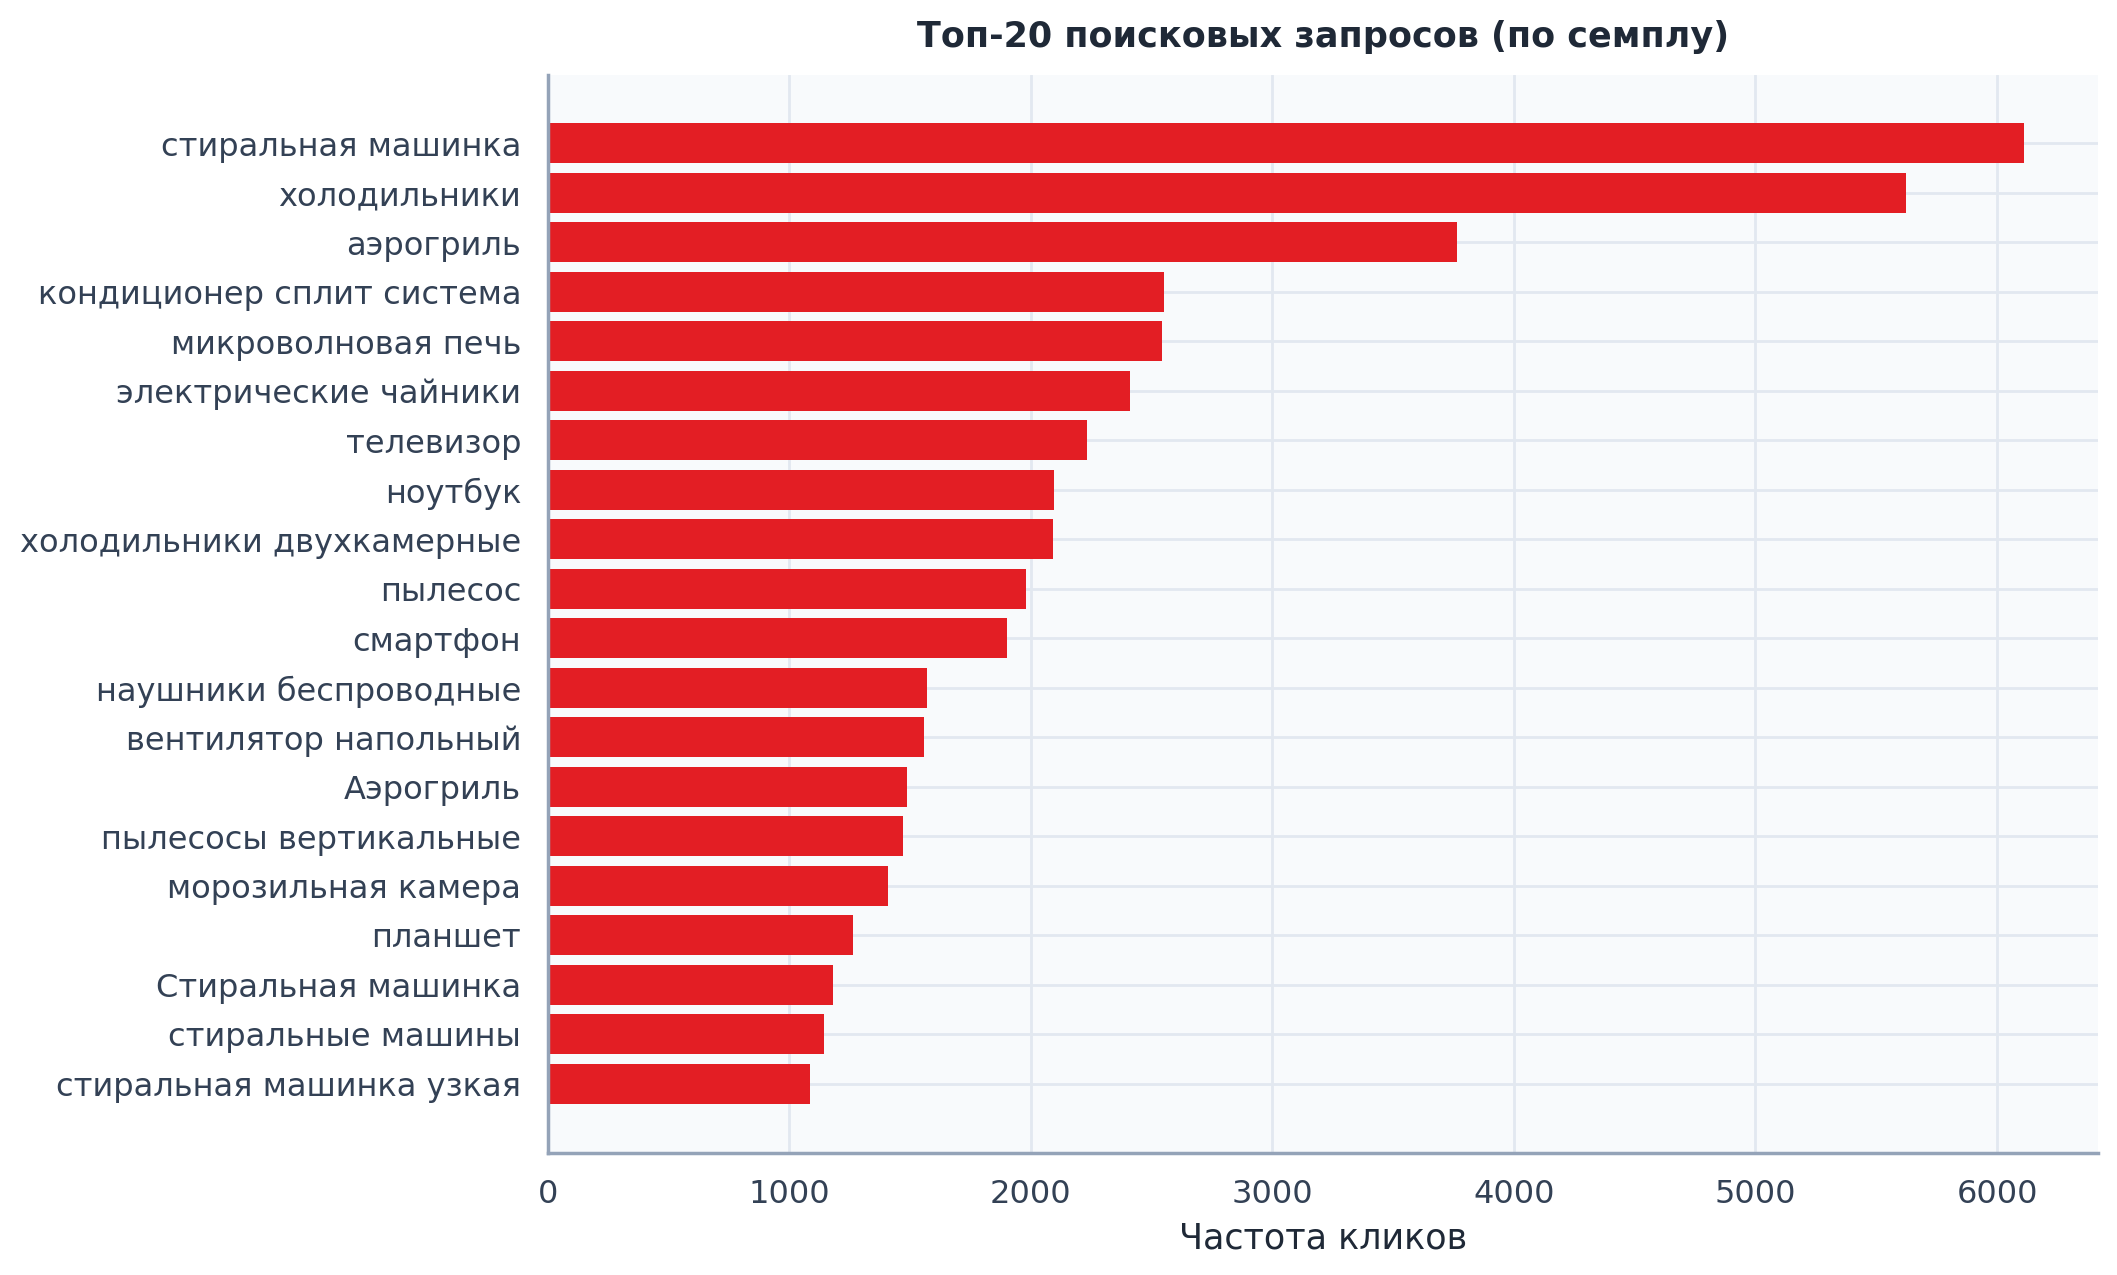
\includegraphics[width=0.94\textwidth]{02_top_queries.png}
\column{0.45\textwidth}
\conclusion{Голова трафика --- категории без бренда: «стиральная машинка», «холодильники», «аэрогриль».}
\vspace{6pt}\par
{\footnotesize
\numdot{1}\ Медианная длина запроса $\approx$ 15--17 символов, 1--3 токена.\par\vspace{4pt}
\numdot{2}\ В топ-15 нет атрибутов: люди уточняют фильтрами или кликами.\par\vspace{4pt}
\numdot{3}\ Категорию надо ловить идеально --- самый частый факт.}
\end{columns}
\slidefoot
\end{frame}

% ============================================================
% 5. EDA: БРЕНДЫ И ЦЕНЫ
% ============================================================
\begin{frame}[t]
\slidehead{eda · бренды и цены}{Бренды: голова мощная, хвост длинный}
\begin{columns}[T]
\column{0.5\textwidth}

\includegraphics[width=\textwidth]{03_top_brands.png}
\column{0.47\textwidth}
\conclusion{Топ-15 брендов покрывает огромную долю кликов, но хвост из 7 тысяч брендов правилами не закрыть.}
\vspace{6pt}\par
{\footnotesize
\numdot{1}\ Apple, Samsung, Haier, Xiaomi --- лидеры кликов.\par\vspace{4pt}
\numdot{2}\ Цены с тяжёлым хвостом: медиана 16 тыс.~₽, средняя 31 тыс.~₽ --- premium тянет вправо.\par\vspace{4pt}
\numdot{3}\ Словарь брендов --- сильный, но конечный инструмент: нужен слой для редких написаний.}
\end{columns}
\slidefoot
\end{frame}

% ============================================================
% 6. EDA: ПОЗИЦИИ КЛИКОВ
% ============================================================
\begin{frame}[t]
\slidehead{eda · клики}{Клики живут в топе выдачи}
\begin{columns}[T]
\column{0.5\textwidth}
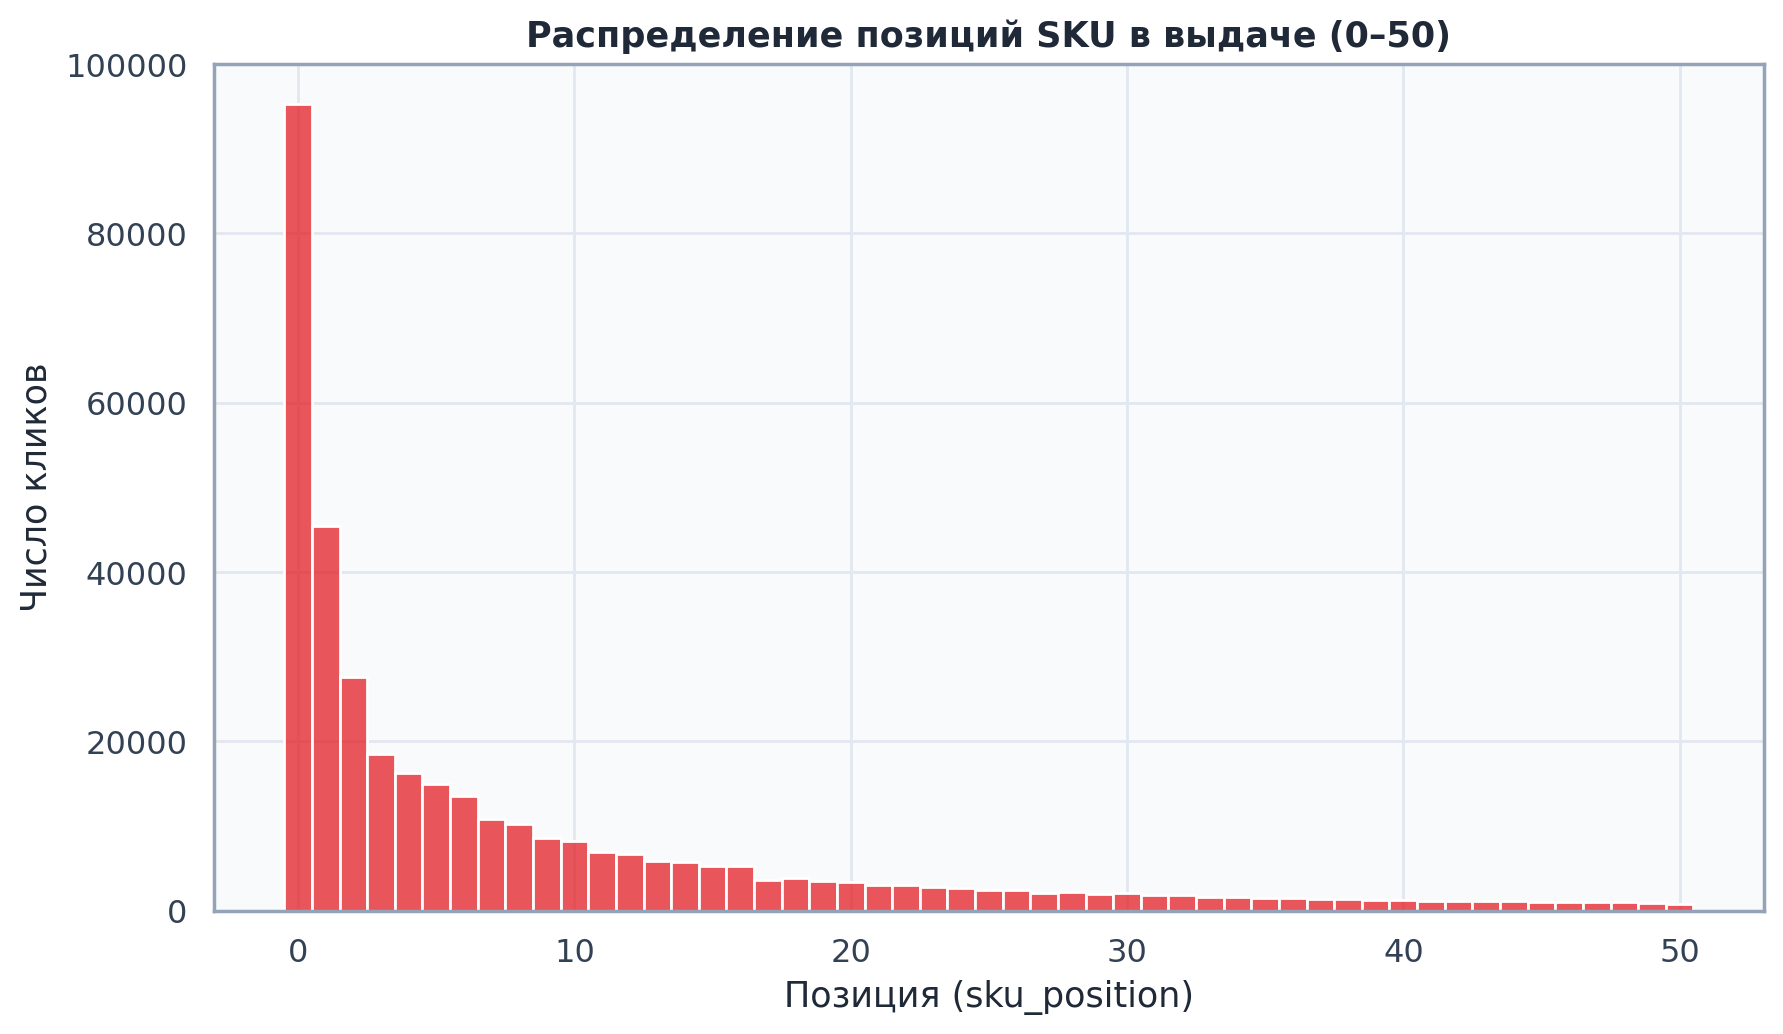
\includegraphics[width=\textwidth]{05_position_distribution.png}
\column{0.47\textwidth}
\conclusion{Медианная позиция клика --- 4. Ошибка разбора запроса почти гарантированно теряет клик.}
\vspace{6pt}\par
{\footnotesize
\numdot{1}\ 75\% кликов --- в первых 16 позициях.\par\vspace{4pt}
\numdot{2}\ Позиция клика --- полезный сигнал качества пары query$\leftrightarrow$SKU (пригодится для разметки match).\par\vspace{4pt}
\numdot{3}\ Связь цены и позиции слабая: дорогие товары кликают и в топе, и глубоко.}
\end{columns}
\slidefoot
\end{frame}

% ============================================================
% 7. ГИПОТЕЗЫ
% ============================================================
\begin{frame}[t]
\slidehead{eda · проверка гипотез}{Гипотезы: что подтвердилось}
{\footnotesize
\renewcommand{\arraystretch}{1.35}
\begin{tabular}{@{}p{7.3cm} p{2.1cm} p{4.2cm}@{}}
\toprule
{\InterSemi Гипотеза} & {\InterSemi Статус} & {\InterSemi Комментарий}\\
\midrule
H1. Большинство запросов --- короткие категорийные интенты & {\color{okgreen}\InterSemi да} & топы --- чистые категории\\
H2. Клики концентрируются в топе выдачи & {\color{okgreen}\InterSemi да} & медиана позиции = 4\\
H3. Бренд в запросе $\Rightarrow$ клик по тому же бренду & {\color{okgreen}\InterSemi в основном} & heatmap query$\times$brand диагональна\\
H4. Цена сильно влияет на позицию клика & {\color{warnorange}\InterSemi нет} & hexbin: связь слабая\\
H5. Атрибуты в запросах пишут единообразно & {\color{warnorange}\InterSemi нет} & «16гб», «16 gb», «16 ГБ» --- зоопарк\\
\bottomrule
\end{tabular}}
\vspace{8pt}\par
\conclusion{H5 --- главный аргумент за вероятностный подход: атрибуты нельзя закрыть одним regex.}
\slidefoot
\end{frame}

% ============================================================
% 8. ПЕРЕПОСТАНОВКА ЗАДАЧИ
% ============================================================
\begin{frame}[t]
\slidehead{постановка · переосмысление}{Задача --- не «обычный NER»}
\conclusion{Главная цель --- максимизировать покрытие edge-cases, а не выбить красивый F1 на простых запросах.}
\vspace{12pt}\par
\begin{columns}[T]
\column{0.48\textwidth}
{\InterSemi\small Почему так}\par\vspace{6pt}
{\small
\numdot{1}\ Голова запросов решается словарём за день --- это не подвиг.\par\vspace{5pt}
\numdot{2}\ Конверсию теряют хвосты: опечатки, редкие бренды, склейки, смесь языков.\par\vspace{5pt}
\numdot{3}\ Ценность решения = сколько хвоста мы покрываем при SLA $<$ 100 мс.}
\column{0.48\textwidth}
\begin{tikzpicture}
\node[fill=cardbg, rounded corners=3pt, inner sep=11pt, text width=\dimexpr\textwidth-22pt\relax]{
{\InterSemi\small Работаем в вероятностном пространстве}\par\vspace{5pt}
{\footnotesize\color{mvgray} Каждый слой отдаёт не только ответ, но и уверенность. Если уверенность низкая --- запрос уходит на слой тяжелее. Так простое остаётся быстрым, а сложное --- решаемым.}
};
\end{tikzpicture}
\end{columns}
\slidefoot
\end{frame}

% ============================================================
% 9. СЛОИСТАЯ АРХИТЕКТУРА
% ============================================================
\begin{frame}[t]
\slidehead{архитектура · слои}{Три слоя: голова, середина, хвост}
\begin{center}
\begin{tikzpicture}[
  lay/.style={rounded corners=3pt, inner sep=10pt, text width=3.55cm, align=left, minimum height=2.9cm},
  arr/.style={-{Stealth[length=2.6mm]}, line width=1pt, mvgray}
]
  \node[lay, fill=cardbg] (l1) at (0,0)
    {{\color{mvred}\InterBold\small ГОЛОВА}\par\vspace{3pt}
     {\InterSemi\footnotesize regex + правила + словари}\par\vspace{4pt}
     {\fontsize{8}{10.5}\selectfont\color{mvgray}частые и простые запросы; мгновенно, прозрачно, дёшево}};
  \node[lay, fill=cardbg] (l2) at (4.75,0)
    {{\color{mvred}\InterBold\small СЕРЕДИНА}\par\vspace{3pt}
     {\InterSemi\footnotesize CRF и аналоги}\par\vspace{4pt}
     {\fontsize{8}{10.5}\selectfont\color{mvgray}token-level: BIO и другие схемы, либо переход к span-level разметке}};
  \node[lay, fill=mvdark] (l3) at (9.5,0)
    {{\color{mvred}\InterBold\small ХВОСТ}\par\vspace{3pt}
     {\color{white}\InterSemi\footnotesize трансформеры + LLM}\par\vspace{4pt}
     {\fontsize{8}{10.5}\selectfont\color{white!75!mvdark}edge-cases, которые не решаются правилами и обычной NER-моделью}};
  \draw[arr] (l1) -- node[above=1pt, font=\fontsize{6.5}{7.5}\selectfont\color{mvgray}, fill=white, inner sep=1.5pt]{низкая увер.} (l2);
  \draw[arr] (l2) -- node[above=1pt, font=\fontsize{6.5}{7.5}\selectfont\color{mvgray}, fill=white, inner sep=1.5pt]{низкая увер.} (l3);
\end{tikzpicture}
\end{center}
\vspace{8pt}\par
\conclusion{Каскад по уверенности: 90\% трафика решают дешёвые слои, тяжёлые модели работают только там, где реально нужны.}
\slidefoot
\end{frame}

% ============================================================
% 10. МАРКОВСКАЯ МОДЕЛЬ
% ============================================================
\begin{frame}[t]
\slidehead{идея · марковская модель}{Марковская цепь для атрибутов}
\begin{columns}[T]
\column{0.5\textwidth}
\conclusion{По предыдущему токену предсказываем тип следующего: после «16» вероятнее всего «гб» --- значит, это memory.}
\vspace{8pt}\par
{\small
\numdot{1}\ Обучаем переходы $P(t_{i+1} \mid t_i)$ на миллионах запросов --- бесплатная статистика.\par\vspace{5pt}
\numdot{2}\ Число без юнита перестаёт быть загадкой: «16» перед «гб» --- память, перед «дюймов» --- диагональ.\par\vspace{5pt}
\numdot{3}\ Дёшево, интерпретируемо, работает в голове каскада рядом с правилами.}
\column{0.46\textwidth}
\begin{tikzpicture}[
  tok/.style={rounded corners=2pt, fill=cardbg, inner sep=7pt, font=\InterSemi\small},
  lab/.style={font=\fontsize{7.5}{9}\selectfont\color{mvred}},
  arr/.style={-{Stealth[length=2.2mm]}, line width=0.9pt, mvred}
]
  \node[tok] (a) at (0,0) {ноутбук};
  \node[tok] (b) at (2.2,0) {asus};
  \node[tok] (c) at (4.0,0) {16};
  \node[tok] (d) at (5.6,0) {гб};
  \draw[arr] (a) -- (b);
  \draw[arr] (b) -- (c);
  \draw[arr] (c) to[bend left=35] node[above, font=\fontsize{7.5}{9}\selectfont\color{mvred}]{$P(\text{гб}\mid 16)$ высокое} (d);
  \node[lab, below=2pt of a] {CATEGORY};
  \node[lab, below=2pt of b] {BRAND};
  \node[lab, below=2pt of c] {ATTR};
  \node[lab, below=2pt of d] {ATTR};
\end{tikzpicture}
\vspace{10pt}\par
\begin{tikzpicture}
\node[fill=pinkband, rounded corners=2pt, inner sep=8pt, text width=\dimexpr\textwidth-16pt\relax]{
{\fontsize{8.5}{11}\selectfont\color{mvdark} attributes: \{«memory»: «16 гб»\} --- юнит восстановлен из контекста, даже если пользователь его не дописал}};
\end{tikzpicture}
\end{columns}
\slidefoot
\end{frame}

% ============================================================
% 11. РАЗМЕТКА MATCH 0/1
% ============================================================
\begin{frame}[t]
\slidehead{идея · разметка match}{Match 0/1: запрос попал в карточку?}
\conclusion{100+ пар размечаем руками: 1 --- клик полностью соответствует запросу, 0 --- иначе. Модель доразмечает остальное.}
\vspace{8pt}\par
\begin{columns}[T]
\column{0.48\textwidth}
{\InterSemi\small Что это даёт}\par\vspace{5pt}
{\footnotesize
\numdot{1}\ «Хорошие запросы» --- кандидаты на улучшение NER: запрос $\approx$ описанию карточки.\par\vspace{4pt}
\numdot{2}\ Чистим шум: «искал айфон $\to$ кликнул чехол» не портит обучение.\par\vspace{4pt}
\numdot{3}\ На метке 1 учим embed(query) $\approx$ embed(title + desc): описание дотаскивает цвет, память, синонимы.}
\column{0.48\textwidth}
{\InterSemi\small Как используем скор}\par\vspace{5pt}
\begin{tikzpicture}[
  st/.style={rounded corners=2pt, fill=cardbg, inner sep=7pt, text width=\dimexpr\textwidth-60pt\relax, font=\fontsize{8}{10.5}\selectfont},
  arr/.style={-{Stealth[length=2.2mm]}, line width=0.9pt, mvgray}
]
  \node[st] (s1) at (0,0) {NER достал факты $\to$ фильтр и буст в выдаче};
  \node[st] (s2) at (0,-0.95) {$P(\text{match}=1 \mid \text{query},\ \text{sku\_text})$ --- реранк поверх};
  \node[st] (s3) at (0,-1.95) {модель: градиентный бустинг (CatBoost / XGBoost) на простых фичах};
  \draw[arr] (s1) -- (s2);
  \draw[arr] (s2) -- (s3);
\end{tikzpicture}
\end{columns}
\slidefoot
\end{frame}

% ============================================================
% 12. ПОДВОДНЫЕ КАМНИ
% ============================================================
\begin{frame}[t]
\slidehead{риски · честно}{Подводные камни и что с ними делать}
{\footnotesize
\renewcommand{\arraystretch}{1.3}
\begin{tabular}{@{}p{4.1cm} p{4.6cm} p{4.6cm}@{}}
\toprule
{\InterSemi Риск} & {\InterSemi Почему больно} & {\InterSemi Решение}\\
\midrule
«Полное соответствие» размыто & «dyson» $\to$ пылесос Dyson --- это 1 или 0? & жёсткий гайд разметки с примерами до старта\\
100 примеров маловато & модель выучит шум выборки & 300--700 меток в день с каждого + проверка согласия\\
Самореференция & модель учится на своих же метках, ошибки размножаются & holdout gold, который модель никогда не размечала\\
Путаница с NER & это про query$\leftrightarrow$SKU, не про BIO на словах & отдельные пайплайны, отдельные метрики\\
\bottomrule
\end{tabular}}
\vspace{8pt}\par
\conclusion{Каждому риску --- конкретный процесс, а не «будем аккуратнее».}
\slidefoot
\end{frame}

% ============================================================
% 13. ПЛАН РАЗМЕТКИ И NEXT STEPS
% ============================================================
\begin{frame}[t]
\slidehead{план · дальше}{План разметки и следующие шаги}
\begin{columns}[T]
\column{0.48\textwidth}
{\InterSemi\small Разметка}\par\vspace{6pt}
{\small
\numdot{1}\ Каждый день от каждого в команде: 300--700 пар вручную.\par\vspace{5pt}
\numdot{2}\ Остальное --- автоматика: правила, алгоритмы, ИИ-агенты с выборочной проверкой глазами.\par\vspace{5pt}
\numdot{3}\ Gold-holdout откладываем сразу и не трогаем до финальной оценки.}
\column{0.48\textwidth}
{\InterSemi\small Следующие шаги}\par\vspace{6pt}
{\small
\numdot{4}\ Марковская модель атрибутов $\to$ в голову каскада.\par\vspace{5pt}
\numdot{5}\ CRF на середину, сравнение BIO vs span-level.\par\vspace{5pt}
\numdot{6}\ Матч-модель (бустинг) на первых 100+ метках $\to$ silver labels $\to$ реранк с description.}
\end{columns}
\vspace{12pt}\par
\conclusion{К защите: каскад с покрытием edge-cases + честные метрики на ручном gold, а не self-check словаря.}
\slidefoot
\end{frame}

% ============================================================
% 14. ФИНАЛ
% ============================================================
\begin{frame}[plain]
\begin{tikzpicture}[remember picture, overlay]
  \fill[mvred] (current page.south west) rectangle (current page.north east);
  \node[anchor=east, inner sep=0pt] at ([xshift=0.32\paperwidth]current page.east)
    {
\includegraphics[height=1.06\paperheight]{kurs1_image1.png}};
  \node[anchor=west, align=left] at ([xshift=0.9cm, yshift=1.2cm]current page.west)
    {\color{white}\InterBold\fontsize{26}{30}\selectfont Спасибо!};
  \node[anchor=west, align=left, text width=0.52\paperwidth] at ([xshift=0.9cm, yshift=-0.35cm]current page.west)
    {\color{white}\fontsize{11}{15}\selectfont Вопросы, критика гипотез и споры про слои --- welcome.};
  \node[anchor=south west] at ([xshift=0.9cm, yshift=0.5cm]current page.south west)
    {\color{white}\fontsize{9}{11}\selectfont День 02 · EDA и гипотезы · Буткемп М.Видео};
\end{tikzpicture}
\end{frame}

\end{document}
